% Example CV based on the 1.5-column-cv template. Main features:
% * uses the Roboto font family and IcoMoon icon set;
% * doesn't use colours, different font weights are used instead for styling;
% * because the CV fits on one page, header and footer is empty, since there isn't much useful info to put there;
% * includes a photo.
\documentclass[a4paper]{article}


% package imports
% ---------------

\usepackage[english]{babel} % for correct language and hyphenation and stuff
\usepackage{calc}           % for easier length calculations (infix notation)
\usepackage{enumitem}       % for configuring list environments
\usepackage{fancyhdr}       % for setting header and footer
\usepackage{fontspec}       % for fonts
\usepackage{geometry}       % for setting margins (\newgeometry)
\usepackage{graphicx}       % for pictures
\usepackage{microtype}      % for microtypography stuff
\usepackage{xcolor}         % for colours
\usepackage{hyperref}       % for document links


\hypersetup {
    colorlinks=false,
}

% margin and column widths
% ------------------------

% margins
\newgeometry{left=10mm,right=10mm,top=10mm,bottom=10mm}

% width of the gap between left and right column
\newlength{\cvcolumngapwidth}
\setlength{\cvcolumngapwidth}{3.5mm}

% left column width
\newlength{\cvleftcolumnwidth}
\setlength{\cvleftcolumnwidth}{45mm}

% right column width
\newlength{\cvrightcolumnwidth}
\setlength{\cvrightcolumnwidth}{\textwidth-\cvleftcolumnwidth-\cvcolumngapwidth}

% set paragraph indentation to 0, because it screws up the whole layout otherwise
\setlength{\parindent}{0mm}


% style definitions
% -----------------
% style categories explanation:
% * \cvnameXXX is used for the name;
% * \cvsectionXXX is used for section names (left column, accompanied by a horizontal rule);
% * \cvtitleXXX is used for job/education titles (right column);
% * \cvdurationXXX is used for job/education durations (left column);
% * \cvheadingXXX is used for headings (left column);
% * \cvmainXXX (and \setmainfont) is used for main text;
% * \cvruleXXX is used for the horizontal rules denoting sections.

% font families
\defaultfontfeatures{Ligatures=TeX} % reportedly a good idea, see https://tex.stackexchange.com/a/37251

\newfontfamily{\cvnamefont}[Path=./Roboto/]{Roboto-Medium}
\newfontfamily{\cvsectionfont}[Path=./Roboto/]{Roboto-Light}
\newfontfamily{\cvtitlefont}[Path=./Roboto/]{Roboto-Regular}
\newfontfamily{\cvdurationfont}[Path=./Roboto/]{Roboto-LightItalic}
\newfontfamily{\cvheadingfont}[Path=./Roboto/]{Roboto-Regular}

\newfontfamily{\regularfont}[Path=./Roboto/]{Roboto-Regular}
\newfontfamily{\italicfont}[Path=./Roboto/]{Roboto-Italic}

\setmainfont[Path=./Roboto/]{Roboto-Light}


% colours
\definecolor{cvnamecolor}{HTML}{000000}
\definecolor{cvsectioncolor}{HTML}{000000}
\definecolor{cvtitlecolor}{HTML}{000000}
\definecolor{cvdurationcolor}{HTML}{000000}
\definecolor{cvheadingcolor}{HTML}{000000}
\definecolor{cvmaincolor}{HTML}{000000}
\definecolor{cvrulecolor}{HTML}{000000}
\definecolor{emphasiscolor}{HTML}{4b5fa3}

\color{cvmaincolor}

% styles
\newcommand{\cvnamestyle}[1]{{\Huge\cvnamefont\textcolor{cvnamecolor}{#1}}}
\newcommand{\cvsectionstyle}[1]{{\normalsize\cvsectionfont\textcolor{cvsectioncolor}{#1}}}
\newcommand{\cvtitlestyle}[1]{{\large\cvtitlefont\textcolor{cvtitlecolor}{#1}}}
\newcommand{\cvdurationstyle}[1]{{\small\cvdurationfont\textcolor{cvdurationcolor}{#1}}}
\newcommand{\cvheadingstyle}[1]{{\normalsize\cvheadingfont\textcolor{cvheadingcolor}{#1}}}

\newcommand{\italicstyle}[1]{{\small\italicfont\textcolor{cvsectioncolor}{#1}}}
\newcommand{\regularstyle}[1]{{\normalsize\regularfont\textcolor{cvsectioncolor}{#1}}}



% inter-item spacing
% ------------------

% vertical space after personal info and standard CV items
\newlength{\cvafteritemskipamount}
\setlength{\cvafteritemskipamount}{2mm plus 1.25mm minus 1.25mm}

% vertical space after sections
\newlength{\cvaftersectionskipamount}
\setlength{\cvaftersectionskipamount}{2mm plus 0.5mm minus 0.5mm}

% extra vertical space to be used when a section starts with an item with a heading (e.g. in the skills section),
% so that the heading does not follow the section name too closely
\newlength{\cvbetweensectionandheadingextraskipamount}
\setlength{\cvbetweensectionandheadingextraskipamount}{1mm plus 0.25mm minus 0.25mm}


% intra-item spacing
% ------------------

% vertical space after name
\newlength{\cvafternameskipamount}
\setlength{\cvafternameskipamount}{3mm plus 0.75mm minus 0.75mm}

% vertical space after personal info lines
\newlength{\cvafterpersonalinfolineskipamount}
\setlength{\cvafterpersonalinfolineskipamount}{1mm plus 0.5mm minus 0.5mm}

% vertical space after titles
\newlength{\cvaftertitleskipamount}
\setlength{\cvaftertitleskipamount}{1mm plus 0.25mm minus 0.25mm}

% value to be used as parskip in right column of CV items and itemsep in lists (same for both, for consistency)
\newlength{\cvparskip}
\setlength{\cvparskip}{0.5mm plus 0.125mm minus 0.125mm}

% set global list configuration (use parskip as itemsep, and no separation otherwise)
\setlist{parsep=0mm,topsep=0mm,partopsep=0mm,itemsep=\cvparskip}

% Set global spacing after each item in itemize
\setlist[itemize]{itemsep=4pt}


% CV commands
% -----------

% creates a "personal info" CV item with the given left and right column contents, with appropriate vertical space after
% @param #1 left column content (should be the CV photo)
% @param #2 right column content (should be the name and personal info)
\newcommand{\cvpersonalinfo}[2]{
    % left and right column
    \begin{minipage}[t]{\cvleftcolumnwidth}
        \vspace{0mm} % XXX hack to align to top, see https://tex.stackexchange.com/a/11632
        \raggedleft #1
    \end{minipage}% XXX necessary comment to avoid unwanted space
    \hspace{\cvcolumngapwidth}% XXX necessary comment to avoid unwanted space
    \begin{minipage}[t]{\cvrightcolumnwidth}
        \vspace{0mm} % XXX hack to align to top, see https://tex.stackexchange.com/a/11632
        #2
    \end{minipage}

    % space after
    \vspace{\cvafteritemskipamount}
}

% typesets a name, with appropriate vertical space after
% @param #1 name text
\newcommand{\cvname}[1]{
    % name
    \cvnamestyle{#1}

    % space after
    \vspace{\cvafternameskipamount}
}

% typesets a line of personal info beginning with an icon, with appropriate vertical space after
% @param #1 parameters for the \includegraphics command used to include the icon
% @param #2 icon filename
% @param #3 line text
\newcommand{\cvpersonalinfolinewithicon}[3]{
    % icon, vertically aligned with text (see https://tex.stackexchange.com/a/129463)
    \raisebox{.5\fontcharht\font`E-.5\height}{\includegraphics[#1]{#2}}
    % text
    #3

    % space after
    \vspace{\cvafterpersonalinfolineskipamount}
}

% creates a "section" CV item with the given left column content, a horizontal rule in the right column, and with
% appropriate vertical space after
% @param #1 left column content (should be the section name)
\newcommand{\cvsection}[1]{
    % left and right column
    \begin{minipage}[t]{\cvleftcolumnwidth}
        \raggedleft\cvsectionstyle{#1}
    \end{minipage}% XXX necessary comment to avoid unwanted space
    \hspace{\cvcolumngapwidth}% XXX necessary comment to avoid unwanted space
    \begin{minipage}[t]{\cvrightcolumnwidth}
        \textcolor{cvrulecolor}{\rule{\cvrightcolumnwidth}{0.3mm}}
    \end{minipage}

    % space after
    \vspace{\cvaftersectionskipamount}
}

% creates a standard, multi-purpose CV item with the given left and right column contents, parskip set to cvparskip
% in the right column, and with appropriate vertical space after
% @param #1 left column content
% @param #2 right column content
\newcommand{\cvitem}[2]{
    % left and right column
    \begin{minipage}[t]{\cvleftcolumnwidth}
        \raggedleft #1
    \end{minipage}% XXX necessary comment to avoid unwanted space
    \hspace{\cvcolumngapwidth}% XXX necessary comment to avoid unwanted space
    \begin{minipage}[t]{\cvrightcolumnwidth}
        \setlength{\parskip}{\cvparskip} #2
    \end{minipage}

    % space after
    \vspace{\cvafteritemskipamount}
}

% typesets a title, with appropriate vertical space after
% @param #1 title text
\newcommand{\cvtitle}[1]{
    % title
    \cvtitlestyle{#1}

    % space after
    \vspace{\cvaftertitleskipamount}
    % XXX need to subtract cvparskip here, because it is automatically inserted after the title "paragraph"
    \vspace{-\cvparskip}
}


% header and footer
% -----------------

% set empty header and footer
\pagestyle{empty}



% preamble end/document start
% ===========================

\begin{document}


% personal info
% -------------

\cvpersonalinfo{
    % photo
    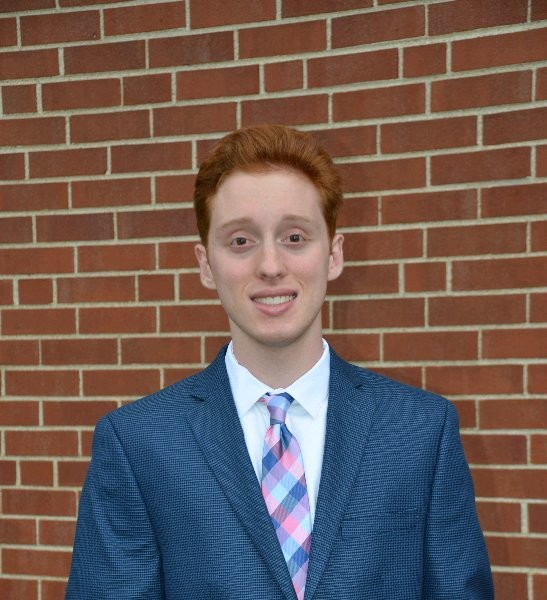
\includegraphics[height=35mm]{img/me.JPG}
}{
    % name
    \cvname{\textcolor{emphasiscolor}{Chris Cohen}}


    % email address
    \cvpersonalinfolinewithicon{height=4mm}{img/email.png}{
      chris@chriscohen.dev
    }

    % LinkedIn account
    \cvpersonalinfolinewithicon{height=4mm}{img/linkedin.png}{
      \href{https://www.linkedin.com/in/cohenchristopher/}{https://www.linkedin.com/in/cohenchristopher/}
    }

    % Website
    \cvpersonalinfolinewithicon{height=4mm}{img/website.png}{
      \href{https://www.chriscohen.dev}{https://www.chriscohen.dev}
    }

    % GitHub
    \cvpersonalinfolinewithicon{height=4mm}{img/github.png}{
      \href{https://github.com/cohenchris}{https://github.com/cohenchris}
    }
}

% education
% ---------

\cvsection{\LARGE \textcolor{emphasiscolor}{EDUCATION}}
\vspace{5mm}

% bachelor's
\cvitem{
    \cvdurationstyle{Aug. 2017 -- May 2021}
}{
  \cvtitle{Bachelor of Science at Purdue University}


    \begin{itemize}[leftmargin=*]
      \item Software Engineering and Cybersecurity
      \item 8x Dean's List, 7x Semester Honors
      \item \large{\regularfont{\textcolor{emphasiscolor}{3.83 GPA}}}
    \end{itemize}
    \vspace{5mm}
}

% work experience
% ---------------

\cvsection{\LARGE \textcolor{emphasiscolor}{EMPLOYMENT}}
\vspace{5mm}

% Qualcomm
\cvitem{
    \cvdurationstyle{May 2021 -- Present}
}{
    \cvtitle{Qualcomm, Secure Systems Group}

    \italicstyle{Software Engineer  --  San Diego, CA}

    \normalsize
    \begin{itemize}[leftmargin=*]
      \item Developed a ROM-backed feature which creates a device-unique, verifiable boot certificate chain (BCC), which attests to the exact state of hardware and software running on the device.
      \item Took full ownership over creating the BCC library, which has been stamped on the Qualcomm Snapdragon SM8650, and 5+ upcoming mobile and automotive chips.
      \item Worked with internal DRM team to use BCC for a new generation of our Remote Key Provisioning feature. This allows for a variety of use-cases, including, including remote provisioning of a device as it leaves the factory, secure video playback, and remote device attestation for customers.
    \end{itemize}
    \vspace{3mm}
}

% Qualcomm Internship
\cvitem{
    \cvdurationstyle{May 2020 -- May 2021}
}{
    \cvtitle{Qualcomm, Government Division (QGOV)}

    \italicstyle{Software Engineering Intern  --  Remote}

    \normalsize
    \begin{itemize}[leftmargin=*]
        \item Developed an Android app for a Qualcomm chipset feature that ensures secure wireless connection,
          communicating information about malicious access points to the user.
    \end{itemize}
}

\vspace{5mm}

% skills
% ------

\cvsection{\LARGE \textcolor{emphasiscolor}{EXPERTISE}}

\vspace{5mm}

% programming languages
\cvitem{
    \cvheadingstyle{Languages}
}{
  C \hspace{12mm} C++ \hspace{12mm} Python \hspace{12mm} ARM/x86 Assembly \hspace{12mm} Bash \hspace{12mm} Javascript
  \vspace{1mm}
}

% topics
\cvitem{
    \cvheadingstyle{Security Clearance}
}{
    \begin{itemize}[leftmargin=*]
      \item \textbf{Secret} clearance through 2024.
      \item Approved for a \textbf{Top Secret} clearance in March 2023.
    \end{itemize}
    \vspace{5mm}
}

% education
% ---------

\cvsection{\LARGE \textcolor{emphasiscolor}{PERSONAL PROJECTS}}
\vspace{5mm}

% Homelab
\cvitem{
    \cvdurationstyle{April 2020 - Present}
}{
  \cvtitle{Home Lab}

    \begin{itemize}[leftmargin=*]
        \item Achieve internal network isolation and security using a custom firewall and 5 VLANs.
        \item Host multiple open-source, privacy-focused services, such as a DNS-level adblocker, email, meta-search engine, and cloud server.
        \item Automate backup of server config and personal files, following the 3-2-1 backup industry standard, allowing for a full restoration using 1 command.
        \item Continuously evaluate network architecture to follow the most bleeding-edge security practices.
    \end{itemize}
}

\end{document}
